\section{Empirical Results and Comparisons}
\label{app:supporting}
\label{app:aligned-xmode}

\subsection{Comparison registry}
\label{app:program-registry}

The primary comparisons cross fresh objective (Dr.GRPO or MaxRL) with
verified replay, first across three model scales on Level 1 and then at
Qwen2.5-0.5B on Level 2. Table~\ref{tab:experiment-map} separates these
comparisons from the supporting controls and replay-weighting ablation.
Terminal populations use the September 11 frozen census. The registered
Qwen2.5-0.5B weighting aggregate retains its original frozen population;
its endpoint values are unchanged in that census.

\begin{table}[H]
  \centering
  \caption{\textbf{Comparison scope and available terminal evidence.}
  A complete block has five registered paired seeds. Primary partial
  intersections retain their exact counts and receive no interval.
  UCPO and sparse RLEP-Dr are reported only at the two smaller model scales;
  their denominators cover all five benchmark domains and five registered
  seeds at each selected scale.}
  \label{tab:experiment-map}
  \label{tab:direct-comparators}
  \scriptsize
  \setlength{\tabcolsep}{3pt}
  \begin{tabularx}{\linewidth}{@{}P{.24\linewidth}P{.20\linewidth}P{.22\linewidth}Y@{}}
    \toprule
    \textbf{Comparison} & \textbf{Scope} & \textbf{Terminal coverage}
      & \textbf{Question} \\
    \midrule
    Dr.GRPO / ReplayDr.GRPO & Level 1, all three scales &
      74/75 pairs; 14/15 complete blocks & Verified memory beyond fresh reward \\
    MaxRL / ReplayMaxRL & Level 1, all three scales &
      67/75 pairs; 12/15 complete blocks & Memory beyond a stronger fresh objective \\
    Four-method factorial & Level 2, Qwen-0.5B &
      4/5 complete domains; two additional Pantry Dr.GRPO pairs & Transfer to harder matched tasks \\
    GRPO & Level 1, all three scales &
      75/75 runs & Reward-standardization control \\
    UCPO & Level 1, 0.5B and 1B &
      50/50 runs & On-policy advantage redistribution \\
    Sparse RLEP-Dr & Level 1, 0.5B and 1B &
      47/50 runs & Success memory without uniform key balancing \\
    Fixed Semantic MaxEnt & Level 1, registered scale/domain blocks &
      10/15 complete blocks & Fresh-rollout semantic exploration \\
    Uniform / frequency replay & Level 1, nine registered blocks &
      43/45 treatment cells; 7/9 complete blocks & Contribution of replay-key balancing \\
    \bottomrule
  \end{tabularx}
\end{table}

\subsection{Terminal comparisons across scales}
\label{app:scale-matrix}
\label{app:scale-snapshot}
\label{app:maxrl-scale-extensions}
\label{app:current-campaign-results}

Within each model--domain--seed comparison, methods share initialization,
data identities, the eight-pass horizon, evaluation requests, verifier, and
replay scheduling code. The replay control runs the same bank and scoring
path with zero replay derivative. Resulting policies can build different
banks. The admissible intersections are defined in
Appendix~\ref{app:source-integrity}.

\crossscaletablematerial

Figure~\ref{fig:maxrl-factorial-scale-extensions} resolves the domain-specific
results behind the main cross-domain display. The 3B MaxRL pairs use
Graph/Countdown/Python/MathIR/Pantry counts $5/3/5/3/1$; the Dr.GRPO pair
uses five seeds except Falcon Countdown, which uses four. These populations
remain separate: a factorial interaction requires the common four-arm
intersection, not differences of aggregates with different seeds.

\begin{figure}[H]
  \centering
  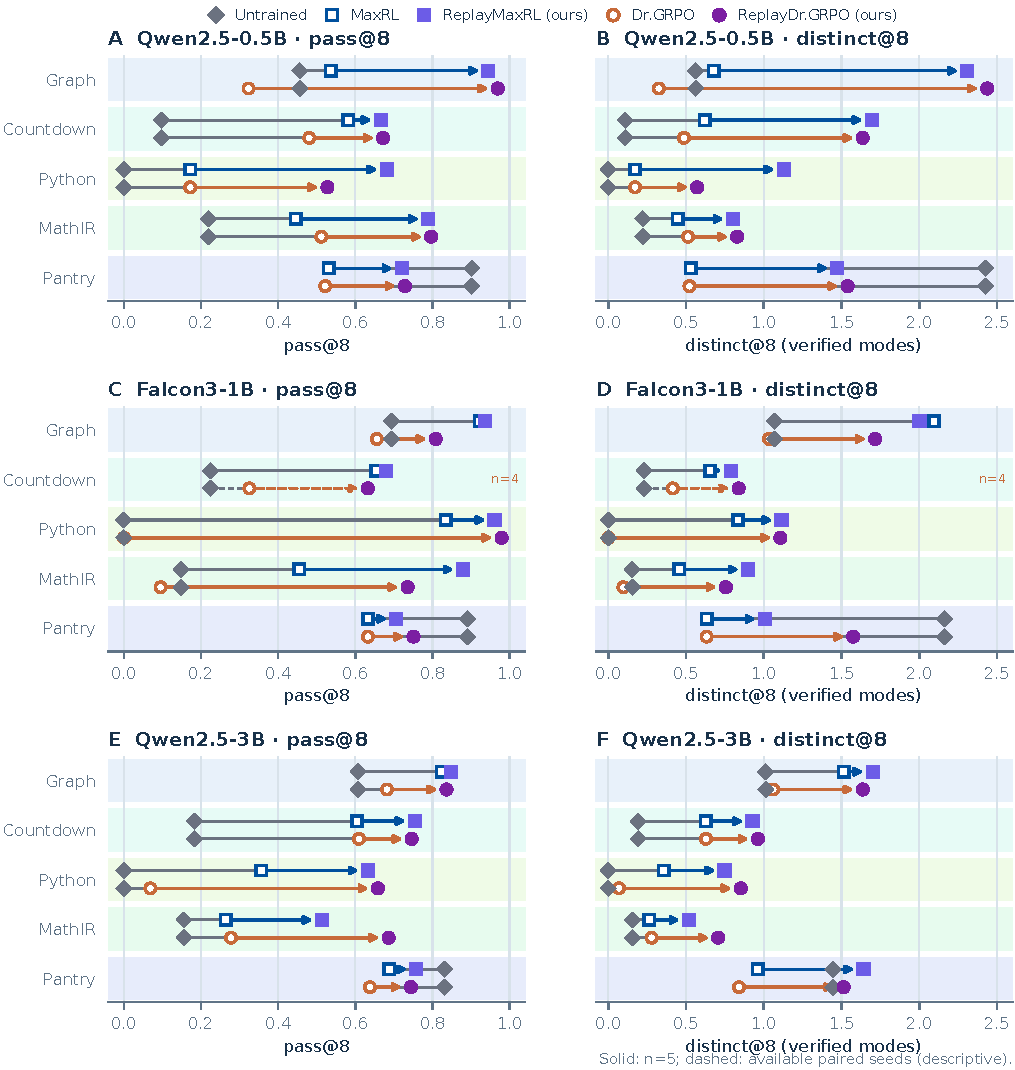
\includegraphics[width=.98\linewidth]
    {figures/e118_scale_extensions_appendix.pdf}
  \caption{\textbf{Per-domain results behind the cross-domain averages in
  Figure~\ref{fig:maxrl-factorial}.} Rows show Qwen2.5-0.5B,
  Falcon3-1B, and Qwen2.5-3B; columns show correctness and raw support.
  MaxRL--ReplayMaxRL pairs retain five terminal seeds throughout the two
  smaller models. Qwen2.5-3B uses $n=5,3,5,3,1$ in domain order;
  dashed connectors mark partial blocks. Dr.GRPO--ReplayDr.GRPO uses four
  admissible seeds for Falcon Countdown and five elsewhere. Domain tints match
  Figure~\ref{fig:modebench-examples}.
  Replay arrows, trained-arm markers, and untrained references use the same
  encoding as the main figure. The
  \href{https://huggingface.co/od2961/maxent-grpo-models/blob/main/experiments/E118/README.md\#models}{E118 model index}
  groups the archived exports by model and domain.}
  \label{fig:maxrl-factorial-scale-extensions}
\end{figure}


Write $P=\texttt{pass@8}$, $D=\texttt{distinct@8}$, and $B=D-P$.
The derived $B$ counts verified modes beyond the first correct outcome in
each sampled set and remains coupled to correctness. The endpoint tables
report exact paired terminal effects. A dash denotes no observed pair;
partial means retain $n/5$ without an interval. Complete-block intervals
are nominal 95\% estimates, without multiple-comparison or repeated-look
adjustment. All underlying arm means and seed effects remain in the
adjacent machine-readable records.

\begin{table}[H]
  \centering
  \caption{\textbf{ReplayMaxRL effects across model scales at pass 8.}
  All effects are ReplayMaxRL minus MaxRL on the displayed paired seeds.
  Brackets give paired Student-$t$ intervals for $\Delta B$ in complete blocks.
  The machine-readable report also retains both arm means, all per-seed
  effects, and intervals for $P$ and $D$.}
  \label{tab:current-e118}
  \scriptsize
  \setlength{\tabcolsep}{3pt}
  \resizebox{\linewidth}{!}{%
  \begin{tabular}{@{}lllcrrr@{}}
    \toprule
    \textbf{Model} & \textbf{Domain} & \textbf{Replay arm} & $n/5$ &
    $\Delta P$ & $\Delta D$ & $\Delta B$ [95\% interval] \\
    \midrule
    % Model & Domain & Contrast & n/5 & Delta P8 & Delta D8 & Delta B8 [95%]
% E118/E119: replay minus base. E120: uniform minus frequency.
% Intervals are stored, descriptive, and only present at n=5.
% E120 dagger: at least one available endpoint pair lacks mechanism eligibility.
Qwen-0.5B & Graph & Re:MaxRL & 5/5 & $+0.408$ & $+1.630$ & $+1.221\;[+0.926, +1.517]$ \\
Qwen-0.5B & Countdown & Re:MaxRL & 5/5 & $+0.084$ & $+1.074$ & $+0.990\;[+0.859, +1.121]$ \\
Qwen-0.5B & Python & Re:MaxRL & 5/5 & $+0.509$ & $+0.955$ & $+0.446\;[-0.156, +1.048]$ \\
Qwen-0.5B & MathIR & Re:MaxRL & 5/5 & $+0.343$ & $+0.356$ & $+0.013\;[+0.008, +0.017]$ \\
Qwen-0.5B & PantryPlan & Re:MaxRL & 5/5 & $+0.189$ & $+0.941$ & $+0.751\;[+0.520, +0.982]$ \\
Falcon-1B & Graph & Re:MaxRL & 5/5 & $+0.014$ & $-0.093$ & $-0.107\;[-0.220, +0.005]$ \\
Falcon-1B & Countdown & Re:MaxRL & 5/5 & $+0.025$ & $+0.133$ & $+0.108\;[+0.082, +0.134]$ \\
Falcon-1B & Python & Re:MaxRL & 5/5 & $+0.127$ & $+0.280$ & $+0.153\;[-0.272, +0.578]$ \\
Falcon-1B & MathIR & Re:MaxRL & 5/5 & $+0.424$ & $+0.443$ & $+0.019\;[+0.006, +0.031]$ \\
Falcon-1B & PantryPlan & Re:MaxRL & 5/5 & $+0.073$ & $+0.375$ & $+0.302\;[+0.034, +0.569]$ \\
Qwen-3B & Graph & Re:MaxRL & 5/5 & $+0.023$ & $+0.186$ & $+0.163\;[+0.021, +0.305]$ \\
Qwen-3B & Countdown & Re:MaxRL & 5/5 & $+0.150$ & $+0.302$ & $+0.152\;[+0.119, +0.185]$ \\
Qwen-3B & Python & Re:MaxRL & 5/5 & $+0.277$ & $+0.391$ & $+0.115\;[+0.080, +0.149]$ \\
Qwen-3B & MathIR & Re:MaxRL & 5/5 & $+0.249$ & $+0.255$ & $+0.006\;[+0.001, +0.011]$ \\
Qwen-3B & PantryPlan & Re:MaxRL & 5/5 & $+0.070$ & $+0.679$ & $+0.609\;[+0.467, +0.751]$ \\
\bottomrule

  \end{tabular}}
\end{table}


At Qwen2.5-0.5B, ReplayMaxRL adds $1.221$, $.990$, and $.751$ extra modes
on Graph, Countdown, and PantryPlan, respectively; each five-seed interval
excludes zero. Falcon Graph instead has a negative mean raw-support effect
($-.093$, interval $[-.229,+.043]$), and its correctness effect is inconclusive
($+.014$, $[-.016,+.044]$). Positive cross-domain effects therefore do not
imply a breadth gain in every domain. The complete Qwen2.5-3B Graph and Python
blocks have positive extra-mode intervals while their correctness intervals
include zero. The three partial 3B domains retain their own seed sets;
the main figure's equally weighted domain average is descriptive.

\subsection{Terminal comparison on the harder level}
\label{app:level2-interim}

Figure~\ref{fig:level2-admission} uses Graph, Countdown, Python, and MathIR:
each has all five seeds at step 3,072 for both levels and all four methods.
Means average those four domains equally within each seed, then the five
seed means. This is a descriptive 20-cell comparison, not a five-domain
estimate; the two levels have separate held-out prompts. At Level 2,
PantryPlan has three Dr.GRPO, three ReplayDr.GRPO, one MaxRL, and one
ReplayMaxRL terminal endpoint. Its only terminal pairs are Dr.GRPO/replay
seeds 43 and 46, with no common four-arm seed. Independently available
arm means do not estimate paired effects.

\begin{table}[H]
  \centering
  \caption{\textbf{Replay effects on the harder Level-2 tasks at pass 8.}
  MaxRL and Dr.GRPO identify the fresh objective; each effect is its replay
  variant minus the corresponding objective without replay. Each row uses
  its own pairwise intersection, which can exceed the four-method
  intersection. Brackets give paired Student-$t$ intervals for $\Delta B$
  only when all five registered pairs are available.}
  \label{tab:current-e119}
  \scriptsize
  \setlength{\tabcolsep}{3pt}
  \resizebox{\linewidth}{!}{%
  \begin{tabular}{@{}lllcrrr@{}}
    \toprule
    \textbf{Model} & \textbf{Domain} & \textbf{Objective} & $n/5$ &
    $\Delta P$ & $\Delta D$ & $\Delta B$ [95\% interval] \\
    \midrule
    % Model & Domain & Contrast & n/5 & Delta P8 & Delta D8 & Delta B8 [95%]
% E118/E119: replay minus base. E120: uniform minus frequency.
% Intervals are stored, descriptive, and only present at n=5.
% E120 dagger: at least one available endpoint pair lacks mechanism eligibility.
Qwen-0.5B & Graph & Dr.GRPO & 5/5 & $+0.561$ & $+1.019$ & $+0.458\;[+0.394, +0.522]$ \\
Qwen-0.5B & Graph & MaxRL & 5/5 & $+0.305$ & $+0.668$ & $+0.363\;[+0.280, +0.446]$ \\
Qwen-0.5B & Countdown & Dr.GRPO & 5/5 & $+0.025$ & $+0.045$ & $+0.020\;[-0.014, +0.055]$ \\
Qwen-0.5B & Countdown & MaxRL & 5/5 & $+0.040$ & $+0.057$ & $+0.017\;[+0.001, +0.032]$ \\
Qwen-0.5B & Python & Dr.GRPO & 5/5 & $+0.075$ & $+0.400$ & $+0.325\;[-0.228, +0.878]$ \\
Qwen-0.5B & Python & MaxRL & 5/5 & $+0.037$ & $+0.212$ & $+0.175\;[-0.295, +0.645]$ \\
Qwen-0.5B & MathIR & Dr.GRPO & 5/5 & $+0.493$ & $+0.493$ & $+0.000\;[+0.000, +0.000]$ \\
Qwen-0.5B & MathIR & MaxRL & 5/5 & $+0.173$ & $+0.175$ & $+0.002\;[-0.003, +0.006]$ \\
Qwen-0.5B & PantryPlan & Dr.GRPO & 2/5 & $+0.234$ & $+0.367$ & $+0.133$ \\
Qwen-0.5B & PantryPlan & MaxRL & 1/5 & $+0.250$ & $+0.404$ & $+0.154$ \\
\bottomrule

  \end{tabular}}
\end{table}


Level-2 Graph provides the clearest replay effects on correctness and extra
modes under both objectives. Countdown's ReplayMaxRL extra-mode effect is
small ($+.017$, interval $[+.001,+.032]$), while its correctness and raw-support
intervals include zero. Python and MathIR have positive mean correctness
and raw-support effects with intervals including zero; MathIR's extra-mode
effects are near zero. Pantry's two-seed Dr.GRPO replay contrast is
$+.234$ on $P$, $+.367$ on $D$, and $+.133$ on $B$, without an interval.

For each common seed and endpoint $Y$, the replay interaction is
\[
 I=(Y^{\rm ReplayMaxRL}-Y^{\rm MaxRL})
    -(Y^{\rm ReplayDr.GRPO}-Y^{\rm Dr.GRPO}).
\]
Replay can add value under both fresh objectives without a positive
interaction. On Level-2 Graph, MaxRL alone raises $P$ relative to Dr.GRPO
by $+.233$ ($[+.140,+.325]$), while the replay interaction on $P$ is
$-.256$ ($[-.329,-.183]$). This is an additional replay benefit after
stronger fresh optimization, without a superadditive interaction.

\begin{table}[H]
  \centering
  \caption{\textbf{Fresh-objective effects and replay interactions on Level 2.}
  All three contrasts within a domain use the same four-arm seed
  intersection. The interaction is
  $(\mathrm{ReplayMaxRL}-\mathrm{MaxRL})-
  (\mathrm{ReplayDr.GRPO}-\mathrm{Dr.GRPO})$.
  Each entry gives its mean and, only for a complete five-seed block, a
  paired unadjusted 95\% Student-$t$ interval. Archived four-arm exports:
  \href{https://huggingface.co/od2961/maxent-grpo-models/blob/main/experiments/E119/README.md\#models}{E119 model index}.}
  \label{tab:level2-factorial-contrasts}
  \scriptsize
  \setlength{\tabcolsep}{3pt}
  \resizebox{\linewidth}{!}{%
  \begin{tabular}{@{}lclrrr@{}}
    \toprule
    \textbf{Domain} & $n$ & \textbf{Contrast} &
    $\Delta P$ & $\Delta D$ & $\Delta B$ \\
    \midrule
    % Domain & paired n & contrast & delta pass@8 & delta distinct@8 & delta extra modes
Graph & 5 & MaxRL $-$ Dr.GRPO & $+.233\;[+.140,+.325]$ & $+.322\;[+.162,+.482]$ & $+.089\;[+.019,+.159]$ \\
Graph & 5 & Re:MaxRL $-$ Re:Dr.GRPO & $-.023\;[-.062,+.016]$ & $-.029\;[-.198,+.140]$ & $-.006\;[-.142,+.130]$ \\
Graph & 5 & Replay $\times$ MaxRL interaction & $-.256\;[-.329,-.183]$ & $-.351\;[-.446,-.255]$ & $-.095\;[-.186,-.003]$ \\
Countdown & 5 & MaxRL $-$ Dr.GRPO & $-.014\;[-.073,+.045]$ & $-.014\;[-.073,+.045]$ & $+.000\;[+.000,+.000]$ \\
Countdown & 5 & Re:MaxRL $-$ Re:Dr.GRPO & $+.002\;[-.008,+.012]$ & $-.002\;[-.047,+.044]$ & $-.004\;[-.042,+.035]$ \\
Countdown & 5 & Replay $\times$ MaxRL interaction & $+.016\;[-.047,+.078]$ & $+.012\;[-.068,+.092]$ & $-.004\;[-.042,+.035]$ \\
Python & 5 & MaxRL $-$ Dr.GRPO & $+.000\;[+.000,+.000]$ & $+.000\;[+.000,+.000]$ & $+.000\;[+.000,+.000]$ \\
Python & 5 & Re:MaxRL $-$ Re:Dr.GRPO & $-.037\;[-.232,+.157]$ & $-.188\;[-.988,+.613]$ & $-.150\;[-1.014,+.713]$ \\
Python & 5 & Replay $\times$ MaxRL interaction & $-.037\;[-.232,+.157]$ & $-.188\;[-.988,+.613]$ & $-.150\;[-1.014,+.713]$ \\
MathIR & 5 & MaxRL $-$ Dr.GRPO & $+.283\;[-.193,+.759]$ & $+.283\;[-.193,+.759]$ & $+.000\;[+.000,+.000]$ \\
MathIR & 5 & Re:MaxRL $-$ Re:Dr.GRPO & $-.036\;[-.158,+.085]$ & $-.035\;[-.158,+.088]$ & $+.002\;[-.003,+.006]$ \\
MathIR & 5 & Replay $\times$ MaxRL interaction & $-.320\;[-.864,+.225]$ & $-.318\;[-.860,+.224]$ & $+.002\;[-.003,+.006]$ \\
PantryPlan & 1 & MaxRL $-$ Dr.GRPO & $+.041$ & $+.061$ & $+.020$ \\
PantryPlan & 1 & Re:MaxRL $-$ Re:Dr.GRPO & $-.021$ & $-.037$ & $-.016$ \\
PantryPlan & 1 & Replay $\times$ MaxRL interaction & $-.062$ & $-.098$ & $-.035$ \\
    \bottomrule

  \end{tabular}}
\end{table}


\subsection{Accuracy and verified modes throughout training}
\label{app:factorial-training-curves}

The following curves include every primary method and model scale used
in the main paper. Each objective pair uses its domain-specific terminal
seed intersection as one fixed cohort throughout training. A checkpoint
is plotted only when all members have complete, valid evaluations for both
methods. Missing or conflicting checkpoints leave gaps; seed counts never
shrink to extend a mean. Four fixed-seed draws of eight samples on the same
128 held-out prompts define each evaluation. Accuracy and mode curves use
identical seeds and checkpoints, without smoothing or outcome-based selection.

\begin{figure}[H]
  \centering
  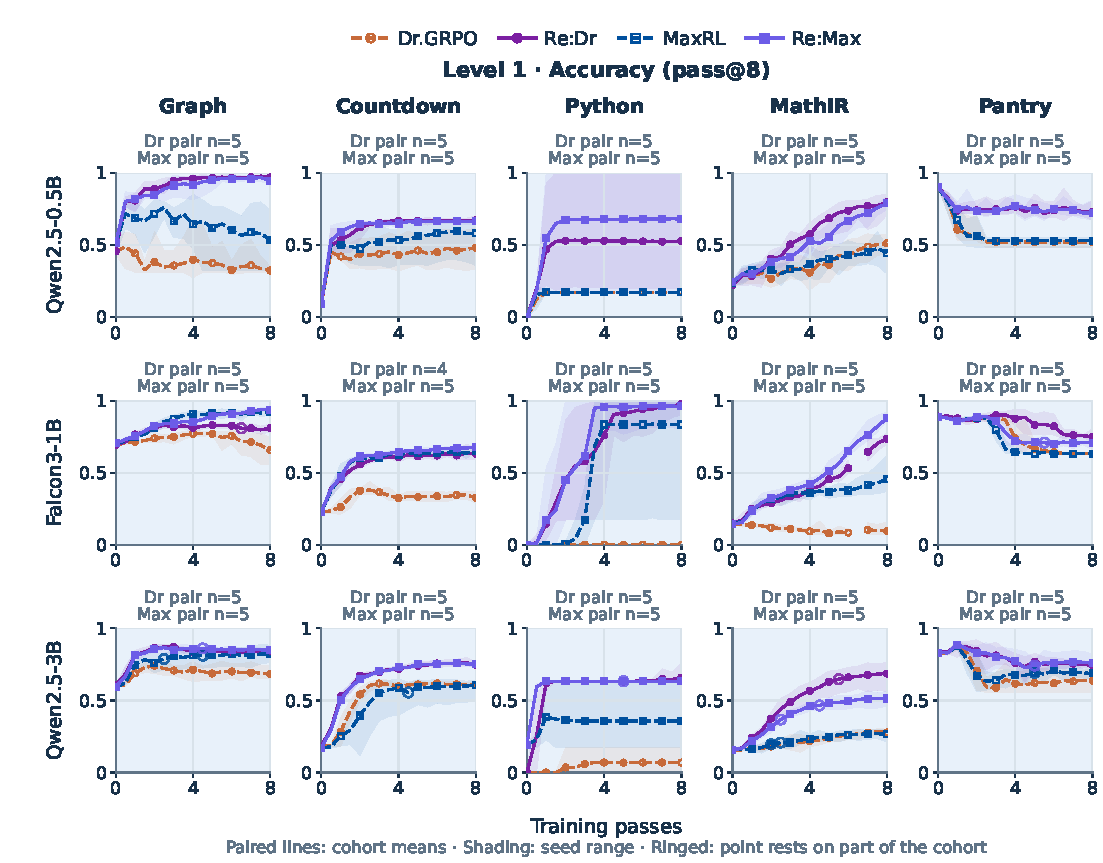
\includegraphics[width=\linewidth]{figures/factorial_training_curves_pass8.pdf}
  \caption{\textbf{Accuracy throughout training at all three model scales.}
  Rows are Qwen2.5-0.5B, Falcon3-1B, and Qwen2.5-3B; columns are the five
  domains. Dr.GRPO, ReplayDr.GRPO, MaxRL, and ReplayMaxRL use the same method
  colors as Figure~\ref{fig:maxrl-factorial}. Lines are fixed-cohort means of
  \texttt{pass@8}; bands are seed ranges, not confidence intervals. Counts
  identify each objective's terminal paired seeds. Qwen2.5-3B MaxRL retains
  Graph/Countdown/Python/MathIR/Pantry counts $5/3/5/3/1$; Falcon Countdown
  Dr.GRPO/replay uses four. Gaps indicate missing or conflicting checkpoints.}
  \label{fig:factorial-training-accuracy}
\end{figure}

\begin{figure}[H]
  \centering
  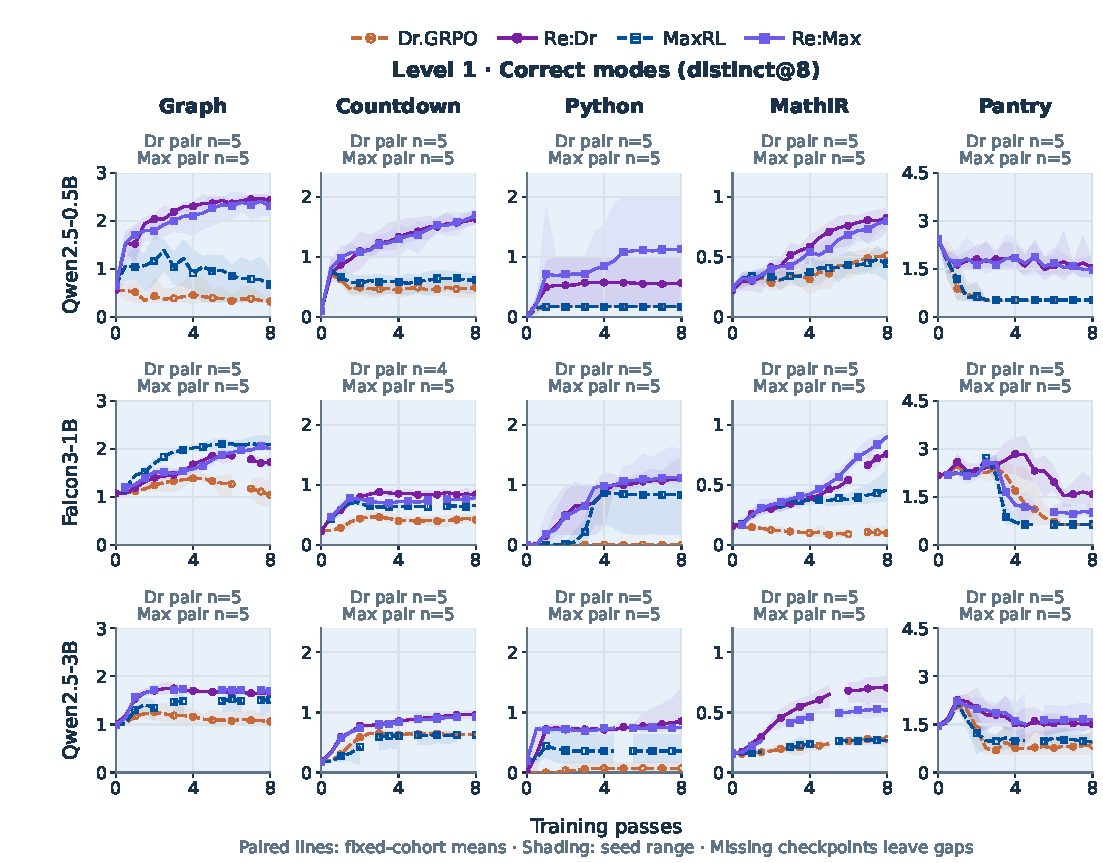
\includegraphics[width=\linewidth]{figures/factorial_training_curves_distinct8.pdf}
  \caption{\textbf{Verified modes throughout training at all three model scales.}
  The same model rows, methods, seeds, and checkpoints as
  Figure~\ref{fig:factorial-training-accuracy}, now measuring
  \texttt{distinct@8}. Lines are descriptive fixed-cohort means and bands
  show seed ranges. A count of one has no band. Domain-specific vertical
  scales are shared across model rows; absolute heights across different
  domains should be read against their labeled axes. Missing evaluations
  are never carried forward or joined across a gap.}
  \label{fig:factorial-training-modes}
\end{figure}

\begin{figure}[H]
  \centering
  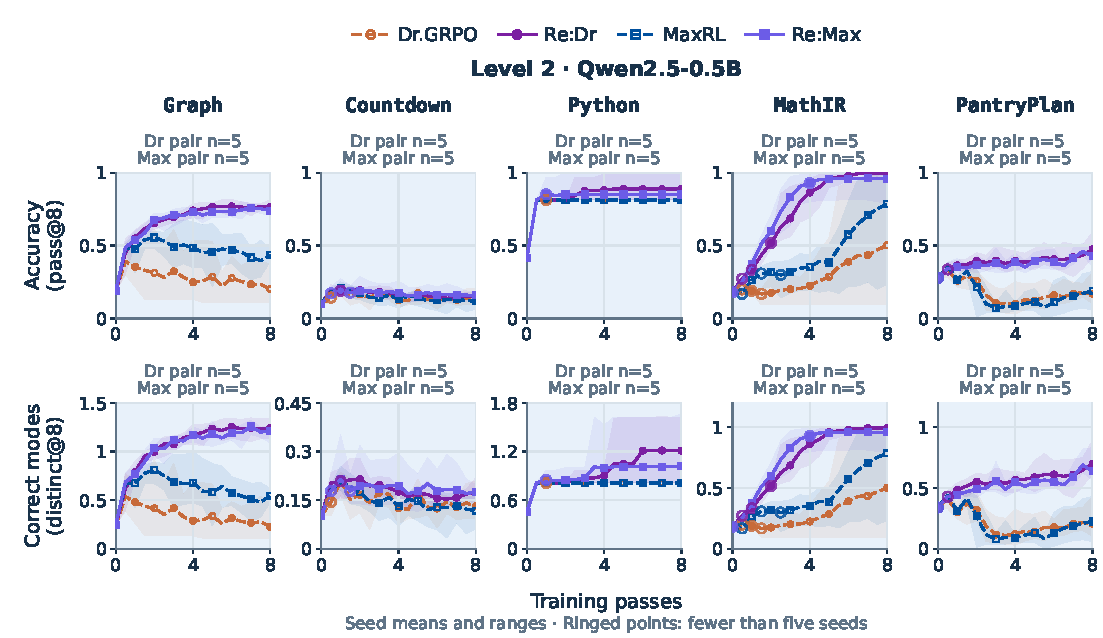
\includegraphics[width=\linewidth]{figures/level2_factorial_training_curves.pdf}
  \caption{\textbf{Accuracy and verified modes during Level-2 training.}
  Qwen2.5-0.5B is the model tested at this level. Rows show \texttt{pass@8}
  and \texttt{distinct@8} for all four primary methods. Graph, Countdown,
  Python, and MathIR contain five terminal paired seeds per objective.
  PantryPlan's Dr.GRPO/replay means use their two terminal paired seeds;
  additional MaxRL and ReplayMaxRL histories are individual, unpaired
  observations, marked separately without a mean or band. They do not
  estimate a paired replay effect. Both metrics follow the same evaluation
  rules, with gaps at missing checkpoints and no extrapolation to later training passes.}
  \label{fig:level2-training-curves}
\end{figure}


\subsection{Supporting comparators}
\label{app:ucpo-progress}

GRPO changes group-reward normalization; UCPO redistributes fresh on-policy
advantage; sparse RLEP-Dr replays verified successes without uniform
canonical-key weighting. Fixed Semantic MaxEnt supplies a fresh-rollout
exploration incentive (Appendix~\ref{app:semantic-maxent}). These are
controls for alternative explanations of the retention results.

\begin{figure}[H]
  \centering
  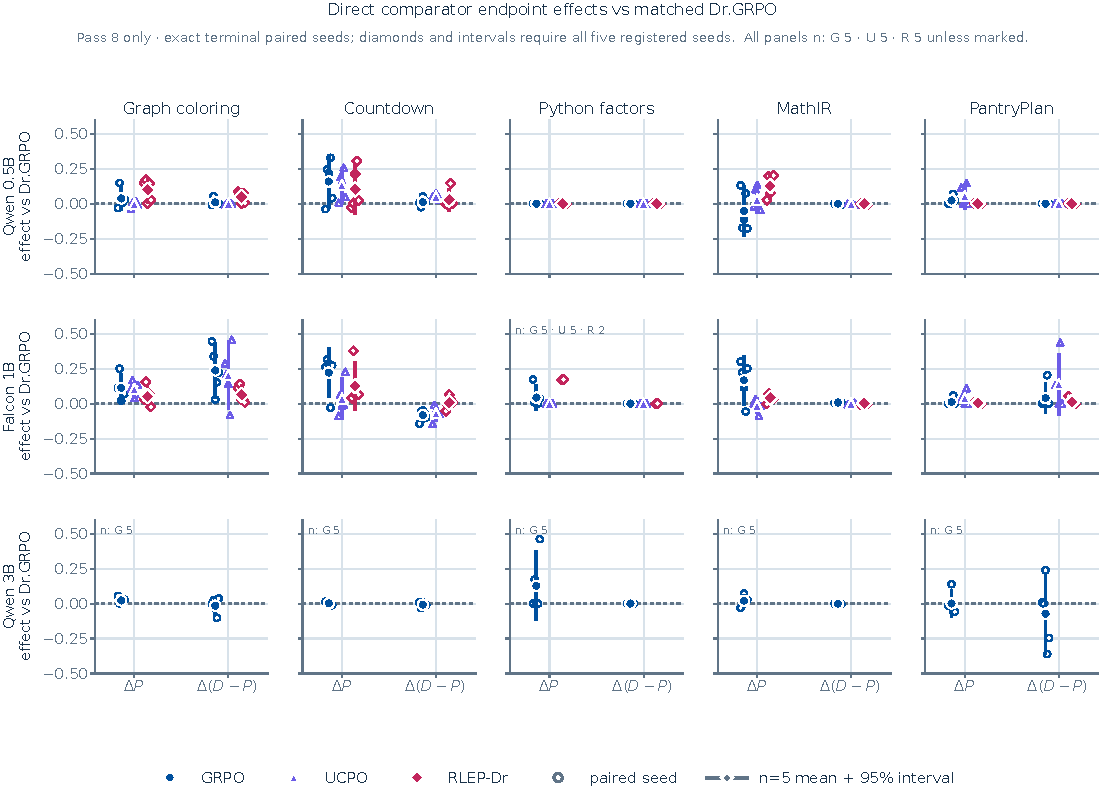
\includegraphics[width=.98\linewidth]
    {figures/direct_comparator_endpoint_effects.pdf}
  \caption{\textbf{Direct alternatives produce local rather than uniform
  final gains.} Each effect subtracts the same-seed Dr.GRPO control
  from the comparator after eight passes. Effects are shown for \texttt{pass@8} and
  correctness-adjusted breadth. Circles are paired seeds; diamonds and 95\%
  Student-\(t\) intervals appear only for complete five-seed blocks. Exact
  \(n\) is printed, and unsupported comparisons remain blank rather than
  being extrapolated or imputed at any seed.}
  \label{fig:direct-comparator-effects}
\end{figure}


The alternatives give local rather than uniform benefits. Qwen-0.5B
Countdown UCPO raises $P$ by $+.133$ ($[+.005,+.262]$) and $B$ by $+.051$
($[+.031,+.071]$), whereas its MathIR effects are inconclusive. MathIR
RLEP-Dr raises $P$ by $+.126$ ($[+.030,+.222]$) with neutral extra modes
($-.002$, $[-.006,+.003]$); its Countdown effects and Falcon Pantry effects
are inconclusive. The full five-seed 3B plain-GRPO blocks likewise have
intervals including zero on both correctness and extra modes.
RLEP's frozen offline pool was collected at temperature $.7$, top-$p=.95$;
all reported evaluations use the common temperature-1, top-$p=1$ contract.
An offline pool versus an online bank remains an algorithmic difference.

\begin{figure}[H]
  \centering
  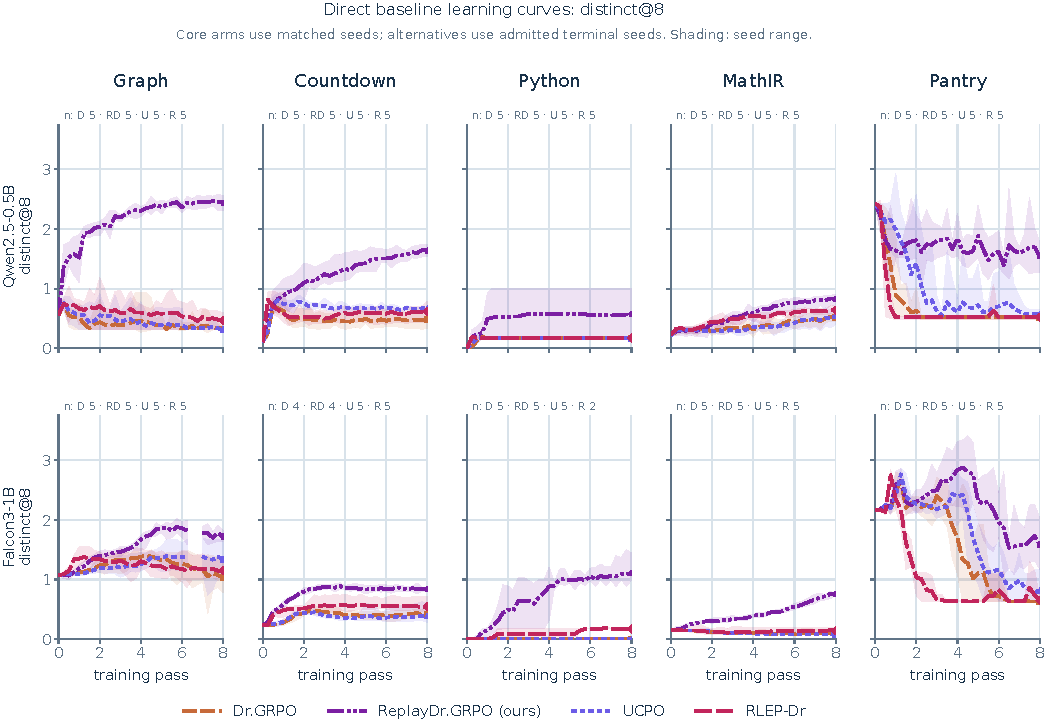
\includegraphics[width=\linewidth]
    {figures/direct_baseline_learning_curves_static_strip.pdf}
  \caption{\textbf{Verified-mode trajectories for the supporting comparators.}
  Rows show Qwen2.5-0.5B and Falcon3-1B; columns are the five domains.
  UCPO and sparse RLEP-Dr are compared with Dr.GRPO and ReplayDr.GRPO
  at these two smaller scales.
  Labels give exact method-specific seed counts. Lines are descriptive
  \texttt{distinct@8} means and bands are seed ranges. The corresponding
  accuracy curves use identical populations in
  Figure~\ref{fig:direct-baseline-accuracy-curves}.}
  \label{fig:direct-baseline-curves}
\end{figure}

\begin{figure}[H]
  \centering
  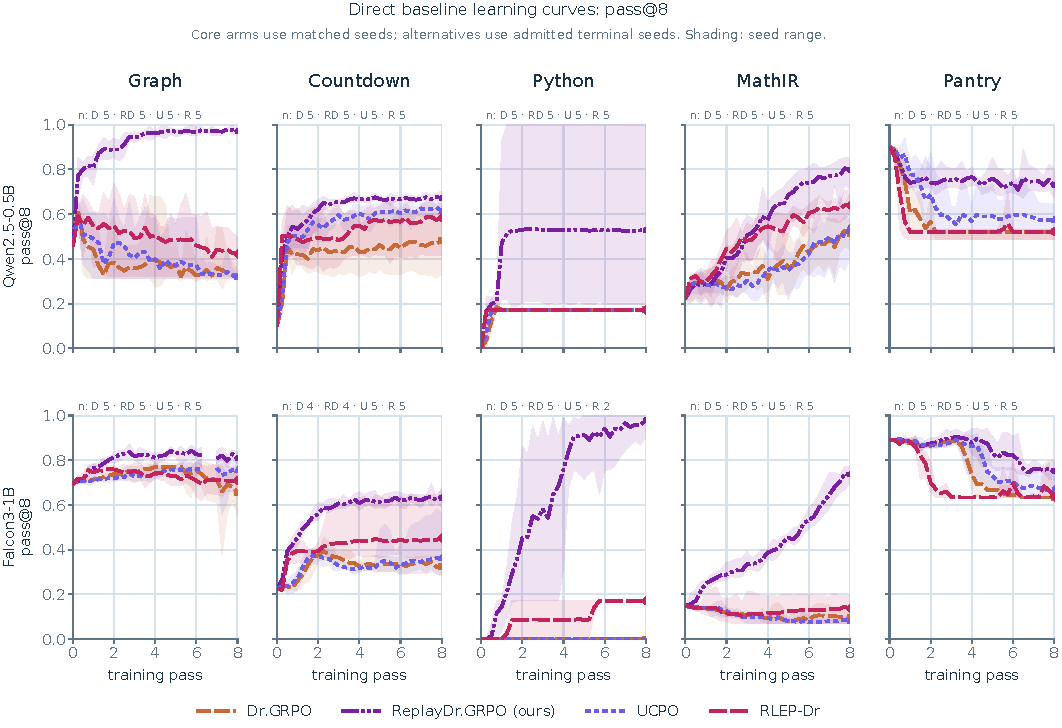
\includegraphics[width=\linewidth]{figures/direct_baseline_learning_curves_pass8.pdf}
  \caption{\textbf{Accuracy trajectories for the supporting comparators.}
  The same model rows, domains, methods, terminal seeds, and registered
  checkpoints as Figure~\ref{fig:direct-baseline-curves}, now measuring
  \texttt{pass@8}. Bands show the seed range and the vertical axes span
  $[0,1]$ throughout. MaxRL and ReplayMaxRL at all three scales are compared
  on both metrics in Figures~\ref{fig:factorial-training-accuracy} and~\ref{fig:factorial-training-modes}.}
  \label{fig:direct-baseline-accuracy-curves}
\end{figure}


\subsection{Uniform versus fresh-frequency replay}
\label{app:frequency-replay-progress}

The weighting ablation retains the same bank construction and update code,
changing only the within-bank target: uniform weights over retained keys
versus weights proportional to validator-positive fresh-rollout counts.
Policy-dependent bank contents can subsequently differ. Positive contrasts
below favor uniform weighting. The registered co-primary contrasts are
$\Delta B$ and $\Delta P$; the five-domain Qwen2.5-0.5B aggregate first
averages domain effects within each matched seed, giving equal domain weight.

Complete-block intervals enumerate all $5^5=3{,}125$ ordered bootstrap
resamples of the five paired training seeds and use linearly interpolated
2.5th and 97.5th percentiles. A resampled seed carries its complete domain
vector when estimating the five-domain aggregate. The endpoints and
aggregate were preregistered; the exact seed-resampling and percentile
conventions are analysis choices. These nominal intervals quantify seed
variability within the fixed benchmark, without resampling prompts or
domains or adjusting across comparisons.

\begin{table}[H]
  \centering
  \caption{\textbf{Uniform versus fresh-frequency replay at pass 8.}
  Effects are uniform minus frequency weighting. Brackets give the paired
  percentile bootstrap interval for $\Delta B$ over all $5^5$ ordered
  resamples in complete blocks. Every observed treatment endpoint in this
  snapshot passes the persisted replay-weight telemetry audit. Partial blocks retain exact seed counts.
  \href{https://huggingface.co/od2961/maxent-grpo-models/blob/main/experiments/E120-R1/README.md\#comparators}{Paired model exports}.}
  \label{tab:current-e120}
  \scriptsize
  \setlength{\tabcolsep}{3pt}
  \resizebox{\linewidth}{!}{%
  \begin{tabular}{@{}lllcrrr@{}}
    \toprule
    \textbf{Model} & \textbf{Domain} & \textbf{Weighting} & $n/5$ &
    $\Delta P$ & $\Delta D$ & $\Delta B$ [95\% interval] \\
    \midrule
    % Model & Domain & Contrast & n/5 & Delta P8 & Delta D8 & Delta B8 [95%]
% E118/E119: replay minus base. E120: uniform minus frequency.
% Intervals are stored, descriptive, and only present at n=5.
% E120 dagger: at least one available endpoint pair lacks mechanism eligibility.
Qwen-0.5B & Graph & Uniform & 5/5 & $+0.066$ & $+0.662$ & $+0.596\;[+0.513, +0.687]$ \\
Qwen-0.5B & Countdown & Uniform & 5/5 & $+0.022$ & $+0.661$ & $+0.639\;[+0.544, +0.733]$ \\
Qwen-0.5B & Python & Uniform & 5/5 & $-0.077$ & $-0.040$ & $+0.037\;[-0.012, +0.123]$ \\
Qwen-0.5B & MathIR & Uniform & 5/5 & $-0.005$ & $+0.014$ & $+0.019\;[-0.001, +0.038]$ \\
Qwen-0.5B & PantryPlan & Uniform & 5/5 & $+0.043$ & $+0.341$ & $+0.298\;[+0.174, +0.400]$ \\
Falcon-1B & Graph & Uniform & 5/5 & $+0.045$ & $+0.278$ & $+0.233\;[+0.182, +0.320]$ \\
Falcon-1B & PantryPlan & Uniform & 5/5 & $-0.021$ & $-0.167$ & $-0.146\;[-0.564, +0.414]$ \\
Qwen-3B & Graph & Uniform & 4/5 & $-0.006$ & $+0.063$ & $+0.070$ \\
Qwen-3B & PantryPlan & Uniform & 5/5 & $+0.011$ & $+0.219$ & $+0.207\;[+0.038, +0.377]$ \\
\bottomrule

  \end{tabular}}
\end{table}


The registered Qwen2.5-0.5B five-domain effect is $+.318$ extra modes per
prompt ($[+.272,+.358]$), with positive within-seed domain averages in all
five seeds. Graph, Countdown, and PantryPlan drive this result; Python and
MathIR remain inconclusive. The correctness effect is $+.010$
($[-.119,+.139]$), establishing neither a gain nor equivalence. Python's
correctness effects range from $-.781$ to $+.828$ across seeds despite
small extra-mode effects in four seeds.

Falcon Graph also favors uniform weighting on extra modes ($+.233$,
$[+.182,+.320]$), but its mean sampled correctness decreases by $-.0152$
($[-.0214,-.0090]$); its $P$ interval includes zero. Falcon Pantry is
inconclusive: $\Delta B=-.146$ ($[-.564,+.414]$) and $\Delta P=-.021$
($[-.063,+.026]$). Qwen2.5-3B Graph and Pantry have descriptive extra-mode
effects of $+.070$ and $+.222$ at four pairs each. All observed treatment
endpoints pass the persisted replay-weight telemetry audit. The evidence
supports a contribution from key balancing in the stated domains, not a
uniform accuracy or breadth advantage across every model--domain block.

\paragraph{Evidence boundary.}
\label{app:scale-boundary}
The primary effects are within-domain, within-scale paired comparisons.
They do not establish a scaling law, a positive factorial interaction, or
preservation of every previously discovered mode. Partial domains are
reported as observed and do not support complete-block generality.
